%% For double-blind review submission, w/o CCS and ACM Reference (max submission space)
\documentclass[sigplan,screen,10pt]{acmart}
\settopmatter{printfolios=true}
%% For double-blind review submission, w/ CCS and ACM Reference
%\documentclass[sigplan,review,anonymous]{acmart}\settopmatter{printfolios=true}
%% For single-blind review submission, w/o CCS and ACM Reference (max submission space)
%\documentclass[sigplan,review]{acmart}\settopmatter{printfolios=true,printccs=false,printacmref=false}
%% For single-blind review submission, w/ CCS and ACM Reference
%\documentclass[sigplan,review]{acmart}\settopmatter{printfolios=true}
%% For final camera-ready submission, w/ required CCS and ACM Reference
%\documentclass[sigplan]{acmart}\settopmatter{}


%% Copyright information
%% Supplied to authors (based on authors' rights management selection;
%% see authors.acm.org) by publisher for camera-ready submission;
%% use 'none' for review submission.
%%% The following is specific to PEPM '20 and the paper
%%% 'GOOL: A Generic Object-Oriented Language'
%%% by Jacques Carette, Brooks MacLachlan, and Spencer Smith.
%%%
\setcopyright{acmlicensed}
\acmPrice{15.00}
\acmDOI{10.1145/3372884.3373159}
\acmYear{2020}
\copyrightyear{2020}
\acmISBN{978-1-4503-7096-7/20/01}
\acmConference[PEPM '20]{Proceedings of the 2020 ACM SIGPLAN Workshop on Partial Evaluation and Program Manipulation}{January 20, 2020}{New Orleans, LA, USA}
\acmBooktitle{Proceedings of the 2020 ACM SIGPLAN Workshop on Partial Evaluation and Program Manipulation (PEPM '20), January 20, 2020, New Orleans, LA, USA}

%% Bibliography style
\bibliographystyle{ACM-Reference-Format}
%% Citation style
%\citestyle{acmauthoryear}  %% For author/year citations
%\citestyle{acmnumeric}     %% For numeric citations
%\setcitestyle{nosort}      %% With 'acmnumeric', to disable automatic
                            %% sorting of references within a single citation;
                            %% e.g., \cite{Smith99,Carpenter05,Baker12}
                            %% rendered as [14,5,2] rather than [2,5,14].
%\setcitesyle{nocompress}   %% With 'acmnumeric', to disable automatic
                            %% compression of sequential references within a
                            %% single citation;
                            %% e.g., \cite{Baker12,Baker14,Baker16}
                            %% rendered as [2,3,4] rather than [2-4].


%%%%%%%%%%%%%%%%%%%%%%%%%%%%%%%%%%%%%%%%%%%%%%%%%%%%%%%%%%%%%%%%%%%%%%
%% Note: Authors migrating a paper from traditional SIGPLAN
%% proceedings format to PACMPL format must update the
%% '\documentclass' and topmatter commands above; see
%% 'acmart-pacmpl-template.tex'.
%%%%%%%%%%%%%%%%%%%%%%%%%%%%%%%%%%%%%%%%%%%%%%%%%%%%%%%%%%%%%%%%%%%%%%


%% Some recommended packages.

\usepackage[utf8]{inputenc}
\usepackage[T1]{fontenc}
\usepackage{microtype}

\usepackage{booktabs}   %% For formal tables:
                        %% http://ctan.org/pkg/booktabs
\usepackage{subcaption} %% For complex figures with subfigures/subcaptions
                        %% http://ctan.org/pkg/subcaption
\usepackage{listings}
\lstset{columns=flexible}

\usepackage{xargs}                      % Use more than one optional parameter 
%in a new commands
\usepackage{pgfplots}
\pgfplotsset{width=9cm,height=6cm,compat=1.8}

\usepackage{balance}
%
% \usepackage[colorinlistoftodos,prependcaption,textsize=tiny]{todonotes}

% for nice TODO notes
% \newcommandx{\unsure}[2][1=]{\todo[inline,linecolor=red,backgroundcolor=red!25,bordercolor=red,#1]{#2}}
% \newcommandx{\change}[2][1=]{\todo[inline,linecolor=blue,backgroundcolor=blue!25,bordercolor=blue,#1]{#2}}
% \newcommandx{\info}[2][1=]{\todo[inline,linecolor=OliveGreen,backgroundcolor=OliveGreen!25,bordercolor=OliveGreen,#1]{#2}}
% \newcommandx{\improvement}[2][1=]{\todo[inline,linecolor=Plum,backgroundcolor=Plum!25,bordercolor=Plum,#1]{#2}}

%%%%%%%%%%%%%%%%%%%%%
%% Useful abbreviations
\newcommand{\Csharp}{C\#}
\newcommand{\Cplusplus}{C\texttt{++}}

\newcommand{\abbrev}[1]{\textbf{#1}}
\newcommand{\mainstream}{\abbrev{mainstream}}
\newcommand{\readable}{\abbrev{readable}}
\newcommand{\idiomatic}{\abbrev{idiomatic}}
\newcommand{\documented}{\abbrev{documented}}
\newcommand{\oopatterns}{\abbrev{patterns}}
\newcommand{\common}{\abbrev{common}}
\newcommand{\expressivity}{\abbrev{expressivity}}

\pagenumbering{gobble}

\begin{document}

%% Title information
\title{GOOL: A Generic Object-Oriented Language}         %% [Short %%Title] is optional;
                                        %% when present, will be used in
%                                        %% header instead of Full Title.
%\titlenote{with title note}             %% \titlenote is optional;
%                                        %% can be repeated if necessary;
%                                        %% contents suppressed with 'anonymous'
%\subtitle{(Short Paper)}                     %% \subtitle is optional
%\subtitlenote{with subtitle note}       %% \subtitlenote is optional;
%                                        %% can be repeated if necessary;
%                                        %% contents suppressed with 'anonymous'


%% Author information
%% Contents and number of authors suppressed with 'anonymous'.
%% Each author should be introduced by \author, followed by
%% \authornote (optional), \orcid (optional), \affiliation, and
%% \email.
%% An author may have multiple affiliations and/or emails; repeat the
%% appropriate command.
%% Many elements are not rendered, but should be provided for metadata
%% extraction tools.

%% Author with single affiliation.
%\orcid{nnnn-nnnn-nnnn-nnnn}             %% \orcid is optional
\author{Jacques Carette}
\orcid{0000-0001-8993-9804}
\affiliation{
%  \position{Position1}
  \department{Department of Computing and Software}              %%
  %%\department is recommended
  \institution{McMaster University}            %% \institution is required
  \streetaddress{1280 Main Street West}
  \city{Hamilton}
  \state{Ontario}
  \postcode{L8S 4L8}
  \country{Canada}                    %% \country is recommended
}
\email{carette@mcmaster.ca}          %% \email is recommended

\author{Brooks MacLachlan}
%\authornote{with author1 note}          %% \authornote is optional;
                                        %% can be repeated if necessary
\affiliation{
  \department{Department of Computing and Software}              %% \department
  \institution{McMaster University}            %% \institution is required
  \streetaddress{1280 Main Street West}
  \city{Hamilton}
  \state{Ontario}
  \postcode{L8S 4L8}
  \country{Canada}                    %% \country is recommended
}
\email{maclachb@mcmaster.ca}          %% \email is recommended

\author{Spencer Smith}
%\authornote{with author1 note}          %% \authornote is optional;
%% can be repeated if necessary
\orcid{0000-0002-0760-0987}
\affiliation{
  \department{Department of Computing and Software}              %%
  \institution{McMaster University}            %% \institution is required
  \streetaddress{1280 Main Street West}
  \city{Hamilton}
  \state{Ontario}
  \postcode{L8S 4L8}
  \country{Canada}                    %% \country is recommended
}
\email{smiths@mcmaster.ca}          %% \email is recommended


%% Abstract
%% Note: \begin{abstract}...\end{abstract} environment must come
%% before \maketitle command
\begin{abstract}
  We present GOOL, a Generic Object-Oriented Language.  GOOL shows that
  with the right abstractions, a language can capture the essence of
  object-oriented programs.  GOOL generates
  human-readable, documented and idiomatic code in 
  Python, Java, \Csharp, and \Cplusplus.
  In it, we can express common programming idioms and patterns.
\end{abstract}


%% 2012 ACM Computing Classification System (CSS) concepts
%% Generate at 'http://dl.acm.org/ccs/ccs.cfm'.
\begin{CCSXML}
<ccs2012>
<concept>
<concept_id>10011007.10011006.10011041.10011047</concept_id>
<concept_desc>Software and its engineering~Source code generation</concept_desc>
<concept_significance>500</concept_significance>
</concept>
<concept>
<concept_id>10011007.10010940.10010971.10011682</concept_id>
<concept_desc>Software and its engineering~Abstraction, modeling and modularity</concept_desc>
<concept_significance>300</concept_significance>
</concept>
<concept>
<concept_id>10011007.10011006.10011008.10011009.10011011</concept_id>
<concept_desc>Software and its engineering~Object oriented languages</concept_desc>
<concept_significance>300</concept_significance>
</concept>
</ccs2012>
\end{CCSXML}

\ccsdesc[500]{Software and its engineering~Source code generation}
\ccsdesc[300]{Software and its engineering~Abstraction, modeling and modularity}
\ccsdesc[300]{Software and its engineering~Object oriented languages}
%% End of generated code


%% Keywords
%% comma separated list
\keywords{Code Generation, Domain Specific Language, Haskell, Documentation}


\maketitle

\section{Introduction}

Java or \Csharp? As languages, this is close to a 
non-question: the two are so similar that only ecosystem issues
would be the deciding factor.  Unlike the question ``C or Prolog?'', which
is almost non-sensical, as the kinds of applications where each
is well-suited are vastly different.  But, given a single
paradigm, such as Object-Oriented (OO), would it be possible to
write a meta-language that captures the essence of writing
OO programs?  They generally all contain (mutable)
variables, statements, conditionals, loops, methods, classes, etc.

OO programs written in different languages appear, superficially,
quite dissimilar. But this is mostly due to
syntactic differences. Are they so different in the utterances that
one can make? Are OO programs akin to sentences in
Romance languages (French, Spanish, Portugese, etc.) which, although 
syntactically different,
are structurally very similar?

This is what we set out to explore.  One non-solution is to pick a
language and implement a translator to the others.
It is feasible --- say by 
engineering a multi-language compiler (such as gcc) to de-compile its Intermediate 
Representation (IR) into most of its input languages.  The end-results would 
be wildly unidiomatic; roughly the equivalent of a novice
in a (spoken) language ``translating'' word-by-word.

So we set out to design a meta-language that embodies
the common semantic concepts of OO languages, encoded so that the
necessary information for translation is present.  This language is
agnostic of the eventual target language -- and free of
the idiosyncratic details of any given language.
In fact, with proper care, one can go even further and
teach the translator about idiomatic patterns of each target language.

Trying to capture all the subtleties of each language is hopeless ---
akin to capturing the rhythm, puns, metaphors, similes,
and cultural allusions of a sublime poem in translation.  But programming
languages are most often used for much more prosaic tasks: writing programs
for getting things done. This is closer to translating technical textbooks,
making sure that all of the meaningful material is preserved.

We want to capture the conceptual meaning of
OO programs, so as to fully automate the translation from
the ``conceptual'' to human-readable, idiomatic code, in mainstream
languages.
At some level, this is not new.  Domain-Specific Languages (DSLs)
are high-level languages with syntax and semantics tailored to a specific
domain~\cite{mernik2005and}.  A DSL
abstracts over the details of ``code'', providing notation to
specify domain-specific knowledge in a natural manner. DSL implementations
often work via translation to a General Purpose programming Language (GPL) for 
execution.  Some generate
human-readable code \cite{wang1997zephyr, mooij2013gaining, hong2012green, 
beyak2011saga}.  This is what we do, for the domain of OO programs.

While designing a generic OO language is a worthwhile endeavour, we had
a second motive: we needed a means to do exactly that as part of
our Drasil project~\cite{Drasil2019, SzymczakEtAl2016}.  The idea of Drasil is
to generate all the requirements documentation and code from expert-provided
domain knowledge.  The generated code needs to be human readable so that
experts can certify that it matches their requirements.
We largely rewrote SAGA~\cite{beyak2011saga} to create
GOOL\footnote{Available at \url{https://github.com/JacquesCarette/Drasil}
as a sub-package.}.
It is implemented as a Haskell embedded DSL (EDSL) that
can currently generate code in Python, Java, \Csharp, and \Cplusplus.
Others can be added, with the implementation effort being commensurate to the
(semantic) distance to the languages already supported.

In Section~\ref{sec:req}, we outline the high-level requirements for GOOL,
followed by an outline of the syntax in Section~\ref{sec:creating}, to
enable concrete examples. The interesting design details are given in
Section~\ref{sec:implementation}. How we capture idioms and patterns is
in Section~\ref{sec:patterns}. We
close with a discussion of related work, plans for future improvements
and conclusions.

\section{Requirements} \label{sec:req}

Our requirements are as follows:

\begin{description}
\item[mainstream] Generate code in mainstream OO languages.
\item[readable] The generated code should be human-readable.
\item[idiomatic] The generated code should be idiomatic.
\item[documented] The generated code should be documented.
\item[patterns] Common OO patterns should be expressible.
\item[expressivity] The language should be rich enough to express a
set of existing OO programs, which act as test cases for the language.
\item[common] Language commonalities should be abstracted.
\end{description}

Targeting OO languages (\mainstream) reflects their popularity,
thus the most potential users --- one reason that the makers
of Scala and Kotlin chose to target the JVM to leverage the Java ecosystem, and
Typescript for Javascript.

The \readable~requirement is not as obvious.  We aim to write
high-level OO code once and have it be available in many GPLs. One use case
is to generate libraries of functions for a narrow domain. As needs
evolve and language popularity changes, it is useful to have it immediately
available in a number of languages. We use it to get \emph{extremely well
documented} code that would be unrealistic to do by hand, as part of
Drasil~\cite{SzymczakEtAl2016, Drasil2019}. \readable~is 
also a proxy for \emph{understandable}, which is helpful for debugging.

The same underlying reasons for \readable~also drive \idiomatic~and \documented,
as they contribute to the human-understandability of the generated code.
\idiomatic~is important as readers would otherwise find the code ``foreign''.
Documentation spans informal one-liners meant for humans to
formal, structured comments for generating API documentation with tools
like Doxygen, or static analysis.
Readability (and thus understandability) are improved when code is 
pretty-printed~\cite{buse2009learning}. Thus layout, redundant parentheses,
well-chosen variable names, and using a common style with lines that are not too
long, are just as useful for generated code as for human-written code.
GOOL does not prevent bad code, it just simplifies creating \readable,
\idiomatic~and \documented~code in multiple languages.

The \oopatterns~requirement is typical of DSLs: common idioms
can be reified into a linguistic form instead of being
informal. Even some of the \emph{design patterns} of~\cite{gamma1995design}
can become part of the language. This makes writing some OO
code even easier in GOOL than in GPLs, but it also helps
keep GOOL language-agnostic and facilitates generating idiomatic code.

\expressivity~is about GOOL capturing
the ideas contained in OO programs.  We test 
GOOL against real-world examples from the Drasil project, such as 
software for determining whether glass withstands a nearby explosion and 
software for simulating projectile motion.

The last requirement (\common) that language commonalities be abstracted, is
internal: we noticed too much code duplication in our initial
backends.

\begin{table*}[t]
  \caption{The GOOL Language - brackets indicate shortcuts for common cases}
  \begin{tabular}{p{2.2cm}| p{15cm}}
    Types & \verb|bool|, \verb|int|, \verb|float|, \verb|char|, 
    \verb|string|, 
    \verb|infile| (read mode), \verb|outfile| (write mode), 
    \verb|listType|, 
    \verb|obj| \\
    Variables & \verb|var|, \verb|extVar|, \verb|classVar|, \verb|objVar|, 
    \verb|$->| (infix operator for \verb|objVar|), \verb|self|,
    [\verb|listVar|] \\
    Values & \verb|valueOf| (value from variable), \verb|litTrue|, 
    \verb|litFalse|, \verb|litInt|, 
    \verb|litFloat|, \verb|litChar|, \verb|litString|, \verb|?!|, 
    \verb|?&&|, 
    \verb|?<|, \verb|?<=|, \verb|?>|, \verb|?>=|, \verb|?==|, \verb|?!=|, 
    \verb|#~|, \verb|#/^|, \verb|#||, \verb|#+|, \verb|#-|, \verb|#*|, 
    \verb|#/|, \verb|#^|, \verb|inlineIf|, \verb|funcApp|, 
    \verb|extFuncApp|, 
    \verb|newObj|, \verb|objMethodCall|, [\verb|selfFuncApp|, 
    \verb|objMethodCallNoParams|] \\
    Statements & \verb|varDec|, \verb|varDecDef|, \verb|assign|, \verb|&=|, 
    \verb|&+=|, \verb|&-=|, \verb|&++|, \verb|&~-|, \verb|break|, 
    \verb|continue|, \verb|returnState|, \verb|throw|, \verb|free|, 
    \verb|comment|, \verb|ifCond|, \verb|ifNoElse|, \verb|switch|, 
    \verb|for|, 
    \verb|forRange|, \verb|forEach|, \verb|while|, \verb|tryCatch|, 
    \verb|block|, \verb|body| [\verb|bodyStatements| (single-block body), 
    \verb|oneLiner| (single-statement body)] \\
    List API & \verb|listAccess|, \verb|at| (same as \verb|listAccess|), 
    \verb|listSet|, \verb|listAppend|, \verb|listIndexExists|, 
    \verb|indexOf|, \verb|listSlice| \\
    Scope & \verb|public|, \verb|private| \\
    Binding & \verb|static_|, \verb|dynamic_| \\
    Functions & \verb|function|, \verb|method|, \verb|param|, 
    \verb|pointerParam|, \verb|mainFunction|, \verb|docFunc|, 
    [\verb|pubMethod|, \verb|privMethod|] \\
    State Variables & \verb|stateVar|, \verb|constVar|, [\verb|privMVar|, 
    \verb|pubMVar| (dynamic), \verb|pubGVar| (static)]\\
    Classes & \verb|buildClass|, \verb|docClass|, [\verb|pubClass|, 
    \verb|privClass|]\\
    Packages & \verb|buildModule|, \verb|fileDoc|, \verb|docMod|, 
    \verb|prog|, 
    \verb|package|, \verb|doxConfig|, \verb|makefile|
  \end{tabular}
  \label{tab:syntax}
\end{table*}

\section{Creating GOOL} \label{sec:creating}

To create a ``generic'' OO language,
we chose an incremental abstraction approach: start from programs written in 
two different languages, and unify them \emph{conceptually}.
We abstract from concrete programs, not just for
\expressivity, but also because that is our ``domain''.  Although
what can be said in any given OO language is quite broad, what we
\emph{actually want to say} is often much more restricted. And what we
\emph{need to say} is often even more concise.
For example, Java offers introspection features, but \Cplusplus~doesn't, so
abstracting from portable OO will not feature introspection (although
generating idiomatic Java may do so). \Cplusplus~templates
are different: while other languages do not necessarily have comparable
meta-programming features, it is not only feasible but easy to provide
template-like features in GOOL, as well as some
partial evaluation. Thus we do not need to generate templates.
We are trying to abstract over the fundamental ideas
expressed via OO programs, rather than abstracting over the languages.
We believe the end result captures the essence of OO programs.
Some features, such as static types, which is not a feature of
Python but required in Java, will be present
as doing full type inference is unrealistic.

Some features of OO programs are not operational: comments and formatting
decisions amongst them.  To us, programs are a bidirectional means of
communication; they must be valid and executable, but
also readable and understandable by humans.
Generating code for interpretation by machines is well understood,
but generating code for human consumption has been given less 
attention. We paid close attention to readability features --- such
as when programmers write long methods, they write them as blocks separated
by blank lines, often with comments.
Thus in GOOL, bodies are not just a sequence of statements, but a 
list of blocks, to represent the actual structure of OO programs.

The GOOL language is shown in Table~\ref{tab:syntax}. We 
distinguish a variable from its value\footnote{as befits the use-mention
distinction from analytic philosophy}, motivated by
semantic considerations; it is beneficial for stricter typing and enables
convenient syntax for \oopatterns~for more idiomatic code.

We might eventually give GOOL its own external syntax, but for now it works
well as a Haskell EDSL, especially as part of Drasil. We can, with judicious
use of smart constructors, somewhat mimic the syntax of OO languages.
We also use smart constructors for common idioms, like
\verb|privMVar| to denote a private dynamic state variable, 
and \verb|pubClass| for a public class.  Note that many of the constructs
(see Table~\ref{tab:syntax}) have \verb|doc| versions.  We can also
generate \verb|Makefile|s and Doxygen config files.

\section{GOOL Implementation} \label{sec:implementation}

There are three standard methods of encoding EDSLs in Haskell:
deep (a set of GADTs), shallow (a set of functions), or ``finally
tagless'' (a set of methods in classes).  GOOL uses a
``sophisticated'' version of tagless~\cite{carette2009finally}
involving \emph{type families}. 

Tagless encodes a language as a generalized
\emph{fold} over any \emph{representation} of the language.  Thus what
look like GOOL ``keywords'' are actually methods, typically 
instantiated to language renderers, but also to static
analysis passes. By using \emph{type families}, each instance can choose
different underlying data structures for GOOL's types.  For example the
\Cplusplus~instance stores destructor statements with state variables, which
is not needed by the other languages.  GOOL is defined by 
$328$ methods across a hierarchy of $43$ classes (see Figure~\ref{fig:classes})
, grouped by functionality --- it is not a small language!

For example, here is part of the class for variables:
\begin{lstlisting}
class (TypeSym repr) => VariableSym repr where
  type Variable repr
  var :: Label -> repr (Type repr)
               -> repr (Variable repr)
\end{lstlisting}
As variables are typed, their representation must be too and
thus that capability (the~\verb|TypeSym| class) is a constraint.  
The \emph{associated type}~\verb|type Variable repr| is a representation-dependent
type-level function.  Each instance can define its own representation of what a
\verb|Variable| is. 

%For Java, we instantiate the \verb|VariableSym| class as follows:
%\begin{lstlisting}
%instance VariableSym JavaCode where
%  type Variable JavaCode = VarData
%  var = varD
%\end{lstlisting}
%where \verb|JavaCode| is essentially the \verb|Identity| monad:
%\begin{lstlisting}
%newtype JavaCode a = JC {unJC :: a}
%\end{lstlisting}
%The \verb|unJC| record field is useful for type inference: when applied to
%an otherwise generic term, it lets Haskell infer that we are wishing
%to only consider the \verb|JavaCode| instances.  \verb|VarData| is defined as
%\begin{lstlisting}
%data VarData = VarD {varBind :: Binding,
%                    varName :: String,
%                    varType :: TypeData,
%                    varDoc :: Doc}
%\end{lstlisting}
%Thus the representation of a (Java) variable consists of more than just its
%printed representation (the \verb|Doc|~field), but also its binding time,
%name, and type of the variable. \verb|Doc| comes from the package 
%\verb|Text.PrettyPrint.HughesPJ| and represents formatted text. It is common 
%in 
%OO programs to declare some variables as \verb|static| to signify that the 
%variable should be bound at compile-time. The \verb|Binding|, either 
%\verb|Static| or \verb|Dynamic|, is thus part of a variable's representation.
%That a variable is aware of its type makes the generation of declarations
%simpler. The inclusion of a name, as a \verb|String|, makes generating
%meta-information, such as for logging, easier.
%
%All representing structures contain at least a \verb|Doc|. It can be considered
%to be our \emph{dynamic} representation of code, from a partial-evaluation
%perspective. The other fields are generally \emph{static} information used to
%optimize the code generation.
%
%We prefer generic code over representation-specific code, so there is little
%code that works on \verb|VarData| directly.  Instead, there are
%methods like \verb|variableDoc|, part of the \verb|VariableSym| type class,
%with signature:
%\begin{lstlisting}
%variableDoc :: repr (Variable repr) -> Doc
%\end{lstlisting}
%which acts as an accessor.  For \verb|JavaCode|, it is simply:
%\begin{lstlisting}
%variableDoc = varDoc . unJC
%\end{lstlisting}
%
%Other uses of additional information are for uniform documentation,
%builds and better arrangement of parentheses.
%Redundant parentheses are typically ignored by 
%compilers, but programmers still tend to minimize them in their code ---
%it makes the code more human-readable. Operator precedence is used for
%this purpose, and thus we also 
%store precedence information in the representations for \verb|Value|s, 
%\verb|UnaryOp|erators and \verb|BinaryOp|erators to elide extra
%parentheses.
%
%Note that the \verb|JavaCode| instance of \verb|VariableSym| defines the
%\verb|var| function via the \verb|varD| function:
%\begin{lstlisting}
%varD :: (RenderSym repr) => Label ->
%  repr (Type repr) -> repr (Variable repr)
%varD n t = varFromData Dynamic n t (varDocD n)
%\end{lstlisting}
%\verb|varD| is generic, i.e. works for all instances, via dispatching to other
%generic functions, such as \verb|varFromData|, which constructs the variable 
%from the pieces in \verb|VarData|. This method is in class 
%\verb|InternalVariable|. Several of these
%``internal'' classes exist, which are not exported from GOOL's interface.
%They contain functions useful for the language renderers, but
%not meant to be used to construct code representations, as they reveal too
%much of the internals (and are rather tedious to use).  One important
%example is the \verb|cast| method, which is never needed by user-level code,
%but frequently used by higher-level functions.

We have defined $300$ functions that abstract over 
\common alities between target languages, making writing new renderers
fairly straightforward. GOOL's Java and \Csharp{} renderers 
show this: out of the $328$ total methods,
$229$ are shared. That is
$40\%$ more common instances than between Python and Java, for example.
A further $37$ are partially shared --- they 
call the same common function but with different parameters. 
\begin{comment}
The numbers of 
common methods between each pair of renderers are shown in 
Figure~\ref{fig:common}. Python is the least 
similar to the other languages, whereas \Csharp has the most in common.
$143$ methods are
the same between all $4$ target languages (which possibly means
they should be generic functions rather than methods).

\begin{figure}[tbh]
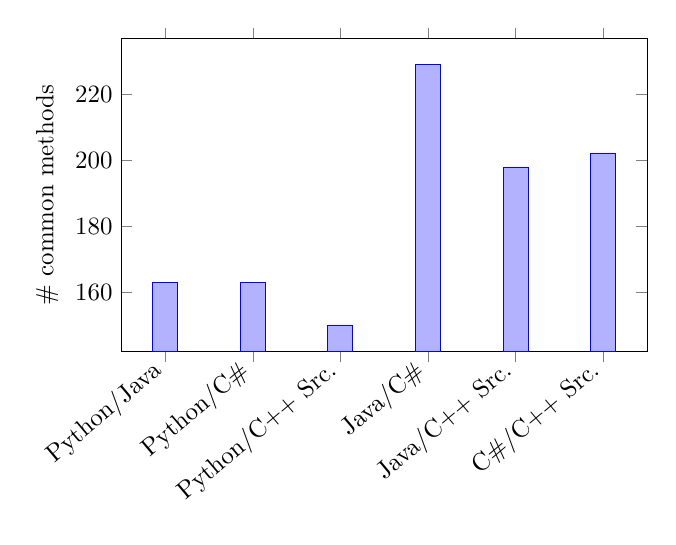
\begin{tikzpicture}[scale=0.9]
\begin{axis}[
ybar,
enlargelimits=0.1,
ylabel={\# common methods},
symbolic x coords={Python/Java,Python/C\#,Python/C++ Src.,Java/C\#,Java/C++ 
Src.,C\#/C++ Src.},
xtick=data,
x tick label style={rotate=40,anchor=east},
]
\addplot coordinates {(Python/Java,163) (Python/C\#,163) (Python/C++ Src.,150) 
(Java/C\#,229) 
(Java/C++ Src., 198) (C\#/C++ Src., 202)};
\end{axis}
\end{tikzpicture}
\caption{Number of common methods between renderers}
\label{fig:common}
\end{figure}
\end{comment}

%\Cplusplus{} is different since most modules are split between a source and
%header file. To generate \Cplusplus, we traverse the code twice,
%once to generate the header file and a second time to generate the
%source file corresponding to the same module. This is done via two instances
%of the classes, for two different types: \verb|CppSrcCode| for source code and
%\verb|CppHdrCode| for header code. Since a main function does not require a
%header file, the \verb|CppHdrCode| instance for a module containing only a main
%function is empty. The renderer optimizes empty modules/files away --- for
%all renderers.
%
%As \Cplusplus{} source and header should always be generated together, a third
%type, \verb|CppCode| achieves this:
%\begin{lstlisting}
%data CppCode x y a = CPPC {src :: x a, hdr :: y a}
%\end{lstlisting}
%The type variables \verb|x| and \verb|y| are intended to be instantiated with
%\verb|CppSrcCode| and \verb|CppHdrCode|, but they are left generic
%so that we may use an even more generic \verb|Pair| class:
%\begin{lstlisting}
%class Pair (p :: (* -> *) -> (* -> *) -> (* -> *)) where
%  pfst :: p x y a -> x a
%  psnd :: p x y b -> y b
%  pair :: x a -> y a -> p x y a
%
%instance Pair CppCode where
%  pfst (CPPC xa _) = xa
%  psnd (CPPC _ yb) = yb
%  pair = CPPC
%\end{lstlisting}
%\verb|Pair| is a \emph{type constructor} pairing, one level up from
%Haskell's own \verb|(,) :: * -> * -> *|.  It is given by one constructor
%and two destructors, much as the Church-encoding of pairs into the
%$\lambda$-calculus.
%
%To understand how this works, here is the instance of \verb|VariableSym|,
%but for \Cplusplus:
%\begin{lstlisting}
%instance (Pair p) => VariableSym 
% (p CppSrcCode CppHdrCode) where
%  type Variable (p CppSrcCode CppHdrCode) = VarData
%  var n t = pair (var n $ pfst t) (var n $ psnd t)
%\end{lstlisting}
%The instance is generic in the pair representation \verb|p| but
%otherwise concrete, because \verb|VarData| is concrete. The actual
%instance code is straightforward, as it just dispatches to the 
%underlying instances, using the generic wrapping/unwrapping
%methods from \verb|Pair|.  This pattern is used for all instances,
%so adapting it to any other language with two (or more) files per
%module is straightforward.

% TODO - bring some back?
\begin{comment}
While ``old'' features of OO languages --- basically features that
were already present in ancestor procedural languages like Algol ---
have fairly similar renderings, more recent (to OO languages) features,
such as for-each loops, show more variations.  More precisely,
the first line of a for-each loop in Python, Java, \Csharp{} and
\Cplusplus~are (respectively):
\begin{lstlisting}
for age in ages:
\end{lstlisting}
\begin{lstlisting}
for (int age : ages) {
\end{lstlisting}
\begin{lstlisting}
foreach (int age in ages) {
\end{lstlisting}
\begin{lstlisting}
for (std::vector<int>::iterator age = ages.begin(); \
  age != ages.end(); age++) {
\end{lstlisting}
where we use backslashes in generated code to indicate manually inserted
line breaks so that the code fits in this paper's narrow column margins. By 
providing \verb|forEach|, GOOL abstracts over these differences.
\end{comment}

\begin{figure}[tp]
\includegraphics[scale=0.289]{GOOLClasses.png}
\caption{Dependency graph of all of GOOL's type classes}
\label{fig:classes}
\end{figure}

\section{Idioms and Patterns} \label{sec:patterns}

\subsection{Idioms}

\paragraph{Command line arguments} Accessing these differs
signficantly across languages.  Thus we abstract over the details through an
\verb|argsList| that represents the list of arguments, with a dedicated API.

\paragraph{Lists}
As with command line arguments, list APIs vary considerably.
We thus reverse engineer the ``useful'' API for lists from actual
use cases.
Lists in OO languages are rarely \emph{linked lists} (unlike Haskell), but
more like dynamically sized vectors. In particular, indexing a list by
position, which is a horrifying idea for linked lists, is extremely common.
The result is a small set of functions and statements, shown in
Table~\ref{tab:syntax} on the line labelled \emph{List API}.

List slicing (the \verb|listSlice|
\emph{statement}) is interesting as the code it generates varies
a lot by language.  For example
\begin{lstlisting}
listSlice someAges (valueOf ages) (Just $ litInt 1) 
  (Just $ litInt 3) Nothing
\end{lstlisting}
in Python is rendered as:
\begin{lstlisting}
someAges = ages[1:3:]
\end{lstlisting}
while in Java it is
\begin{lstlisting}
ArrayList<Double> temp = new ArrayList<Double>(0);
for (int i_temp = 1; i_temp < 3; i_temp++) {
    temp.add(ages.get(i_temp));
}
someAges = temp;
\end{lstlisting}
Idiomatic code generation is enabled by having
appropriate high-level information driving the generation.

\paragraph{Printing}
is also target dependent.  Again Python
is more ``expressive'' so that printing a list (via
\verb|printLn ages|) generates \verb|print(ages)|, but in other languages
we must generate a loop. 
% for example, in \Cplusplus:
% \begin{lstlisting}
% std::cout << "[";
% for (int list_i1 = 0; list_i1 < \
%   (int)(myName.size()) - 1; list_i1++) {
%   std::cout << myName.at(list_i1);
%   std::cout << ", ";
% }
% if ((int)(myName.size()) > 0) {
%   std::cout << myName.at((int)(myName.size()) - 1);
% }
% std::cout << "]" << std::endl;
% \end{lstlisting}
There is also similar functionality for reading input.

\paragraph{Procedures with I/O/B parameters}
Our hand-written target codes had methods that
used their parameters differently: as inputs, outputs, or both.
This is a \emph{semantic} pattern that is
not necessarily obvious in any of the implementations. Once noticed,
we created an encoding of that information to generate better,
more idiomatic code.  Concretely, the following Python code
\begin{lstlisting}
def applyDiscount(price, discount):
    price = price - discount
    isAffordable = price < 20

    return price, isAffordable
\end{lstlisting}
can be captured in GOOL with the \verb|inOutFunc| idiom:
\begin{lstlisting}
inOutFunc "applyDiscount" public static_
  [discount] [isAffordable] [price]
  (bodyStatements [
    price &-= valueOf discount,
    isAffordable &= valueOf price ?< litFloat 20.0])
\end{lstlisting}
We can produce the following \Csharp
\begin{lstlisting}
public static void applyDiscount(ref int price, \
  int discount, out Boolean isAffordable) {
    price = price - discount;
    isAffordable = price < 20;
}
\end{lstlisting}
and \Cplusplus
\begin{lstlisting}
void applyDiscount(int &price, \
  int discount, bool &isAffordable) {
    price = price - discount;
    isAffordable = price < 20;
}
\end{lstlisting}
to capture the same idea.  The Java version (not shown) is more
awkward.
A natural task-level ``feature'' --- 
different kinds of parameters --- ends up being rendered differently,
but hopefully idiomatically, in each target language.  GOOL manages the
tedious aspects of generating any needed variable declarations and return
statements.  To call an \verb|inOutFunc| function, one must use
\verb|inOutCall| so that GOOL can ``line up'' all the pieces properly.

\paragraph{Getters and setters} are common in OO programs (regardless of
whether these actually achieve encapsulation), and mechanical to write.
In GOOL, \verb|getMethod "FooClass" foo| and \verb|setMethod "FooClass" foo|
are sufficient to generate that code, which can be called with
\verb|get| and \verb|set|, and yet abstracts over the idiosyncracies of
each target language.

\paragraph{Design Patterns}
GOOL currently handles three design patterns: Observer,
State, and Strategy~\cite{gamma1995design}. 

For Strategy, we ensure that the set of
strategies that will be used are statically known at generation
time, and then generate code only for those that will
be used.  \verb|runStrategy| is the user-facing function.

For Observer, \verb|initObserverList| generates an observer, given a list
of initial values; it generates a declaration of
an observer list variable, initially containing the given values.
\verb|addObserver| can be used to add a value to the observer list, and
\verb|notifyObservers| will call a method on each of the observers. Currently,
the name of the observer list variable is fixed, so there can only be one
observer list in a given scope.

The State pattern is specialized to \emph{Finite State Machines}
with fairly general transition functions.  Transitions happen on checking, not
on changing the state. \verb|initState| takes a name and a state label and
generates a declaration of a variable.
\verb|changeState| changes the state of the variable.
\verb|checkState| is more complex:  it takes the name of the state variable, a
list of value-body pairs, and a fallback body; it generates a conditional
(usually a switch statement) that checks the state and runs the corresponding
body, or the fallback body, if none of the states match.

The design patterns could have been coded in GOOL, but
having these as language features is useful for two reasons: 1) the GOOL-level
code is clearer in its intent (and more concise), and 2) the resulting code
can be more idiomatic.

Figure~\ref{fig:code} shows a larger example.  The recommended style is
to name all strings (to avoid hard-to-debug typos) and variables, then
write the code proper.
\begin{figure}[tb]
\begin{lstlisting}
patternTest :: (MethodSym repr) =>
  repr (Method repr)
patternTest = let      fsmName = "myFSM"
 offState = "Off"      onState = "On"
 noState = "Neither"   obsName = "Observer"
 obs1Name = "obs1"     obs2Name = "obs2"
 printNum = "printNum" nName = "n"
 obsType = obj obsName
 n = var n int
 obs1 = var obs1Name obsType
 obs2 = var obs2Name obsType
 newObs = extNewObj obsName obsType [] in
   
 mainFunction (body [block [
  varDec n,

  initState fsmName offState, 
  changeState fsmName onState,
  checkState fsmName 
  [(litString offState, 
         oneLiner $ printStrLn offState), 
   (litString onState, 
         oneLiner $ printStrLn onState)] 
  (oneLiner $ printStrLn noState)],

  block [
   varDecDef obs1 newObs, 
   varDecDef obs2 newObs],

  block [
   initObserverList obsType [valueOf obs1], 
   addObserver $ valueOf obs2,
   notifyObservers (func printNum void []) obsType]])
\end{lstlisting}
\caption{GOOL sample code}
\label{fig:code}
\end{figure}

\section{Related Work} \label{sec:related}

\subsection{General-Purpose Code Generation}

\textbf{Haxe}~\cite{Haxe} is a general-purpose multi-paradigm language and cross-platform
compiler.  It compiles to all of the languages GOOL does, and many
others.  However, it is designed as a more traditional programming language, and
does not offer the high-level abstractions that GOOL provides. Furthermore
Haxe strips comments and generates source code around a custom framework; 
the effort of learning this framework and the lack of comments makes the generated
code not particularly readable. The internal organization of Haxe does not seem
to be well documented.

\textbf{Protokit}~\cite{kovesdan2017multi} is a DSL and code generator for Java and
\Cplusplus, where the generator is designed to produce
general-purpose imperative or object-oriented code. The Protokit generator is
model-driven and uses a final ``output model'' from which actual code can be
generated. Since the ``output model'' is quite similar to the generated
code, it presented challenges with regards to semantic, conventional, and
library-related differences between the target languages
\cite{kovesdan2017multi}. GOOL's design helps overcome differences between
target languages.

\textbf{ThingML}~\cite{harrand2016thingml} is a DSL for model-driven engineering
targeting C, \Cplusplus, Java, and JavaScript. It is specialized to deal with
distributed reactive systems (a nevertheless broad range of application domains).
This means that it is not quite a general-purpose DSL, unlike GOOL.
ThingML's modelling-related syntax and abstractions stand in contrast to GOOL's
object-oriented syntax and abstractions. The generated code lacks some of the
pretty-printing provided by GOOL, specifically indentation, which detracts from
readability.

\subsection{Object-Oriented Generators}

There are code generators which multiple target OO languages, but all are
domain-specific.

\textbf{Google protocol buffers}~\cite{Protobuf} is a DSL for serializing
structured data, which can be compiled into Java, Python, Objective C, and
\Cplusplus.  \textbf{Thrift}~\cite{slee2007thrift} is a Facebook-developed tool
for generating code in multiple languages and even multiple paradigms based on
language-neutral descriptions of data types and interfaces.
\textbf{Clearwater}~\cite{swint2005clearwater} is an approach for implementing
DSLs with multiple target languages for components of distributed systems.  The
\textbf{Time Weaver} tool~\cite{de2004glue} uses a multi-language code
generator to generate ``glue'' code for real-time embedded systems.  The domain
of mobile applications is host to a bevy of DSLs with multiple target
languages, of which \textbf{MobDSL}~\cite{kramer2010mobdsl} and
\textbf{XIS-Mobile}~\cite{ribeiro2014xis} are two examples.
\textbf{Conjure}~\cite{Conjure} is a DSL for generating APIs. It reads YML
descriptions of APIs and can generate code in Java, TypeScript, Python, and
Rust.

\subsection{Design Patterns}

A number of languages for modeling design patterns have been developed. The
\textbf{Design Pattern Modeling Language} (DPML)~\cite{mapelsden2002design} is similar
to the Unified Modeling Language (UML) but designed specifically to overcome
UML's shortcomings. DPML consists of
both specification diagrams and instance diagrams for instantiations of design
patterns, but does not attempt to generate actual source code.
The \textbf{Role-Based Metamodeling Language}~\cite{kim2003uml} is also based on UML but
with changes to allow for better models of design patterns, with specifications
for the structure, interactions, and state-based behaviour in patterns. Again,
source code generation is not attempted. Another metamodel for design patterns
includes generation of Java code~\cite{albin2001meta}. IBM developed a DSL in 
the form of a visual user interface for generation of OO code based on design 
patterns~\cite{budinsky1996automatic}. The languages that
generate code do so only for design patterns, not for any general-purpose code,
as GOOL does.

\section{Future Work} \label{sec:future}

Currently GOOL code is typed based on what it represents:
variable, value, type, or method, for example. The type system does not
go ``deeper'', so that values (such as booleans
and strings) are simply ``values''.  This is sufficient to allow us to
generate well-formed code, but not to ensure that it is well-typed.
We have started to statically type GOOL.

We also want to improve the generated import statements, via tracking
actual dependencies on features used.  In general, we can do various 
kinds of static analyses to enhance the code generation quality,
such as being more precise about \verb|throws Exception| in Java.

We also want to interface with external libraries, such as a variety of ODE
solvers, since Drasil currently focuses on scientific applications. The API for
available solvers varies considerably, so we will need to change the ``shape''
of generated code depending on the user's choice.

Some implementation decisions, such as representing lists in Java as 
\verb|ArrayList|, are hard-coded. But we could have used \verb|Vector| instead.
We would like such a choice to be user-controlled. Another such decision
point is to allow users to choose which specific external library to use.

\section{Conclusion} \label{sec:conclusions}

We currently successfully use GOOL to simultaneously generate code in all of 
our target languages for the glass and projectile programs described in Section 
\ref{sec:req}. 

Conceptually, mainstream object-oriented languages are similar enough that it
is indeed feasible to create a single ``generic'' object-oriented language that
can be ``compiled'' to them.  Of course, these languages are syntactically
quite different in places, and each contains some unique ideas as well.
In other words, there exists a ``conceptual'' object-oriented language that
is more than just ``pseudocode'': it is a full-fledged executable language
that captures the common essence of mainstream OO
languages.

GOOL is an unusual DSL, as its ``domain'' is actually that of object-oriented
programs. More precisely, of conceptual programs that can be
easily written in languages containing a procedural core with an
object-oriented layer on top --- which is what Java, Python, \Cplusplus{}, and
\Csharp{} are.

Since we are capturing \emph{conceptual programs}, we can achieve
several things that we believe are \emph{together} new:
\begin{itemize}
\item generation of idiomatic code for each target language,
\item turning coding patterns into language idioms,
\item generation of human-readable, well-documented code.
\end{itemize}

We must also re-emphasize this last point: that for GOOL, the generated code
is meant for human consumption as well as for computer consumption. This is
why semantically meaningless concepts such as ``blocks'' exist: to be able
to chunk code into pieces meaningful for the human reader, and provide
documentation at that level as well.

%% Acknowledgments
%\begin{acks}                            %% acks environment is optional
                                        %% contents suppressed with 'anonymous'
  %% Commands \grantsponsor{<sponsorID>}{<name>}{<url>} and
  %% \grantnum[<url>]{<sponsorID>}{<number>} should be used to
  %% acknowledge financial support and will be used by metadata
  %% extraction tools.
%\end{acks}


%% Bibliography
\balance
\bibliography{References}


%% Appendix
% \appendix
% \section{Appendix}
% 
% Text of appendix \ldots
% 
\end{document}
